\documentclass[a4paper,twoside,master.tex]{subfiles}
\begin{document}
\lecture{26}{Wednesday, March 25, 2020}{Derivatives of the Partition Function}

\begin{align}
    \pdv{\beta} \ln{Z} &= \frac{1}{Z} \pdv{Z}{\beta} = \frac{1}{Z} \pdv{\beta} \int \frac{\dd[3N]{p} \dd[3N]{q}}{h^{3N} N!} e^{- \beta H(p,q)} \\
    &= \int \dd[3N]{p} \dd[3N]{q} (- H(p,q)) \underbrace{\frac{e^{- \beta H(p,q)}}{Z h^{3N} N!}}_{\text{canonical state}} \\
    &= - \ev{H(p,q)}_{\text{CS}}
\end{align}
so
\begin{equation}
    E \equiv \ev{H} = - \pdv{\beta}\ln Z = \pdv{\beta} \left( \beta F \right)
\end{equation}

Can we learn anything new aside from simply reproducing the thermodynamics we already know? Yes, but we need to go to higher derivatives. Recall that
\begin{equation}
    c_V = \frac{T}{N} \eval{\pdv{S}{T}}_{V,N} = \frac{1}{N} \eval{\pdv{E}{T}}_{V,N}
\end{equation}
Notice that $ T \dd{S} = E $ in this scenario, so

\begin{align}
    c_V &= \frac{1}{N} \pdv{T} \ev{H} = \frac{1}{N} \pdv{\beta}{T} \pdv{\beta} \ev{H} = - \frac{\beta}{NT} \pdv{\beta} \ev{H} \\
    &= - \frac{\beta}{TN} \pdv{\beta} \frac{\int \frac{\dd[3N]{p} \dd[3N]{q}}{h^{3N} N!} H(p,q) e^{- \beta H(p,q)}}{\int \frac{\dd[3N]{p} \dd[3N]{q}}{h^{3N} N!} e^{- \beta H(p,q)}}
\end{align}
To simplify this notation, let us introduce the following:
\begin{equation}
    \Tr( \cdot ) := \int \frac{\dd[3N]{p} \dd[3N]{q}}{h^{3N} N!} ( \cdot )
\end{equation}
Using this notation,
\begin{align}
    c_V &= - \frac{\beta}{TN} \pdv{\beta} \frac{\Tr(H e^{- \beta H})}{\Tr(e^{- \beta H})} \\
    &= - \frac{\beta}{TN} \frac{\Tr(-H^2 e^{- \beta H}) \Tr(e^{- \beta H}) - \Tr(H e^{- \beta H}) \Tr(-H e^{- \beta H})}{\left[ \Tr(e^{- \beta H}) \right]^2} \\
    &= - \frac{\beta}{TN} \left[ \frac{\Tr(-H^2 e^{- \beta H})}{\Tr(e^{- \beta H})} + \left( \frac{\Tr(H e^{- \beta H})}{\Tr(e^{- \beta H})} \right)^2 \right] \\
    &= \frac{\beta}{TN} \left[ \ev{H^2} - \ev{H}^2 \right] \\
    &= \frac{\beta}{TN} \sigma^2_H
\end{align}
It turns out that this heat capacity can be written as a resultt of fluctuations of the Hamiltonian!
\begin{equation}
    \underbrace{\sigma^2_H}_{\text{energy fluctuations}} = \underbrace{N}_{\text{extensive}} \underbrace{(k_B T)}_{\text{characteristic energy}} \underbrace{\frac{c_V}{k_B}}_{\text{response function}} 
\end{equation}
This is an example of a ``fluctuation-response theorem''. It is generally beyond thermodynamics because it talks about fluctuations\textemdash something we talk about in statistical physics.

\begin{figure}[h]
    \centering
    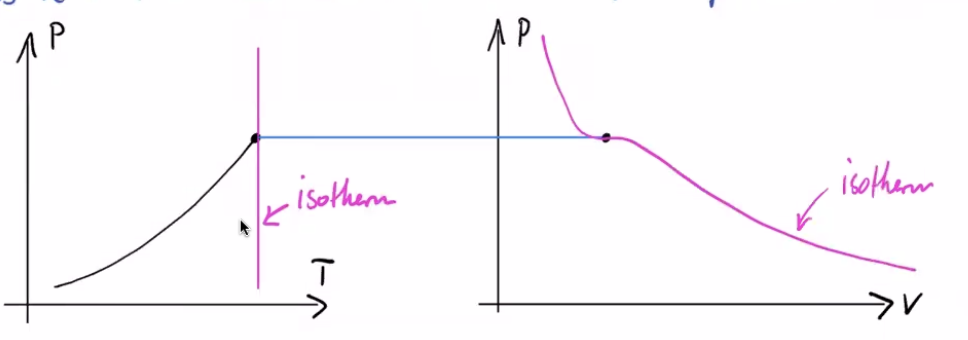
\includegraphics[width=\textwidth]{figures/lec_26_critical_point.png}
    \caption{Plot of an Isotherm through the Critical Point}
    \label{fig:lec_26_critical_point}
\end{figure}
Notice that $ \sigma_H^2 \sim N $, as expected from our last lecture. Can response functions be infinite? It certainly seems mathematically possible. Imagine an isotherm through a critical point of a phase transition. At the critical point, $ \eval{\pdv{P}{V}}_{T} = 0 $, so $ \kappa_T = \infty $ (see \Cref{fig:lec_26_critical_point}). In fact, most response functions (compressibility, specific heat, etc.) tend to diverge at critical points. However, this would seem to suggest that $ \sigma_H^2 = \infty $ at these points, so how is this even possible? We happen to know that probability densities with infinite variance exist (Cauchy-Lorentz) and they have some curious properties. At the critical point, the system shows fluctuations that are not Gaussian (because the Central Limit Theorem no longer holds)!\ This is the beginning of some awesome physics which unfortunately are beyond the scope of this class.

\end{document}
